% ********** Software platform **********

\chapter{Software platform}

The software that runs on the Sparrowv3 nodes and the SparrowDongle was
developed by As. Drd. Ing. Andrei Voinescu and is known as the SparrowLibrary.
In the process of implementing this protocol we have greatly improved not only
its functionality but its stability and its ease of use.

The main focus of this library is to provide a C interface for working with the
Sparrow nodes and dongle. It must also be compatible with past and future
Sparrow devices, thus it must support multiple platforms and do this in a
scalable and maintainable manner. To this end we divided the library into board
and platform sections.  Each device must declare exactly one board and one
platform, with the board defining the physical components that make up the
device (sensors, LEDs etc.) and the platform defining the microcontroller (ADC,
timers etc.). 

In order to facilitate switching between different devices we used a
cross-platform build system (CMAKE) and divided the library into modules. The
build system allows the user to select the device that his/her code is to be
compiled for. Makefiles will be automatically generated to suit. Modularization
of the library means that new code can be easily added, while keeping the
compilation process fast and the resulting code efficient.

Next we will present some of the most important modules in the library and
their implementation.

\section{Microcontroller}

This module contains the microcontroller initialization function. The purpose
of this function is to take the controller to the most energy efficient state
possible. In the case of the \mbox{ATmega128RFA1} this means disabling power to
peripherals. Power will be re-enabled to a peripheral by its controlling
module's initialization function, if called. This means any unused modules will
be turned off not drain any power.

The function also enables data retention on all SRAM blocks. This is a special
configuration that the \mbox{ATmega128RFA1} requires in order to be able to
use deep sleep states without suffering data loss.

\section{Radio}

This module allows the user to enable the \mbox{ATmega128RFA1} radio
transceiver and use it in either a non-interactive or an interactive way. 

The interactive interface consists of a series of functions that can be called
to manipulate the device. They allow the user to put the transceiver into sleep
state or into active mode, to check its availability for accepting new commands
and to transmit and receive a frame (both blocking and non-blocking).

The programmer can also choose to work with the radio in a non-interactive
manner. This is achieved through four callbacks that can be passed to the
initialization function and which are automatically called by interrupts that
the transceiver generates: a wake-up callback, a reception start callback, a
reception end callback and a transmission end callback.

\begin{figure}[ht]
	\begin{center}
		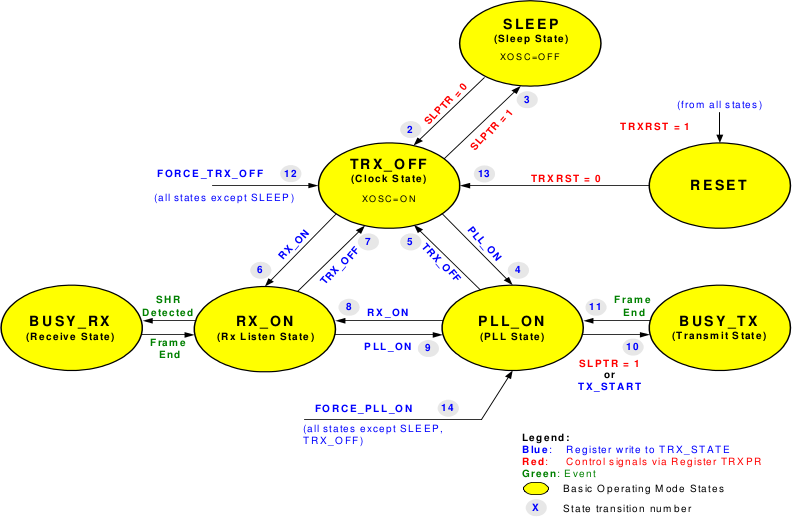
\includegraphics[width=\textwidth]
		{img/transceiver_operating_modes.png}
	\end{center}
	\caption{\small \itshape{Transceiver operating
	modes\protect\footnotemark}}
	\label{fig:transceiver_operating_modes}
\end{figure}
\footnotetext{Image taken from \mbox{ATmega128RFA1} datasheet. Copyright 2012
Atmel Corporation.}

The two methods of interaction allow for different application designs.  The
device can be easily integrated in both procedural and event-based systems.

The \mbox{ATmega128RFA1} radio transceiver has 7 operating modes, as shown is
figure \ref{fig:transceiver_operating_modes}. The user can trigger a state
transition by using the \emph{radio\_set\_state} and
\emph{radio\_set\_state\_force} functions. The difference between the two is
that the latter forces the transceiver to the \emph{TRX\_OFF} state, triggers a
new transition to the desired state and then waits until the unit enters that
state, thus assuring that after the function returns the transceiver is in the
desired state.

After microcontroller initialization the transceiver is powered off. The radio
initialization enables power to it and puts it into sleep mode. It can be
woken-up by using the \emph{radio\_wake\_up} function. After the transition
from the \emph{SLEEP} to \emph{TRX\_OFF} state has ended (i.e. the unit has
completed the wake-up) the wake-up callback is triggered. The transceiver can
be put back to sleep using the \emph{radio\_sleep} function.

Frames are sent using the \emph{radio\_send\_frame} and
\emph{radio\_send\_frame\_block} functions, the former being non-blocking and
the latter blocking. They can only be called when the transceiver is not in
sleep mode. They will force the unit into the \emph{PLL\_ON} state, load data
into the frame buffer and issue the transmission start command. The module uses
double-buffering for frame data. There is an application frame buffer and a
transceiver frame buffer. Data is transferred between the two buffers before
transmitting a frame and after receiving a new frame. The transceiver will
transition back to the \emph{PLL\_ON} state after the transmission is complete
and it will trigger the transmission end callback.

Receiving a frame is done by calling the \emph{radio\_receive\_frame} function,
which is non-blocking, or its blocking counterpart,
the \emph{radio\_receive\_frame\_block} function. To enable reception the
transceiver is forced into the \emph{RX\_ON} state. It will now transition to
the \emph{BUSY\_RX} state upon detecting a valid SHR (synchronization header).
This also triggers the reception start callback. After the frame end is
detected the transceiver transitions back to the \emph{RX\_ON} state and the
reception end callback is triggered.

\section{Symbol counter}

The symbol counter module provides an interface for enabling and interacting
with the \mbox{ATmega128RFA1} MAC symbol counter, which is used as the primary
time source in Sparrow-based applications. It allows the user to set two
independent timeouts as large as 4294967296 seconds and put the microcontroller
to sleep for up to 4294967296 milliseconds. As with the radio, the symbol
counter module provides two callbacks that are triggered when one of the two
timeouts expires.

An example of using the symbol counter to schedule time critical work is show
in listing \ref{lst:time_critical_work}.

\lstset{
	language=C, numbers=none, caption=Time critical work snippet,
	label=lst:time_critical_work
}
\begin{lstlisting}
#define TIMEOUT	30

void timeout_callback()
{
	do_time_critical_work();
	scounter_set_timeout(TIMEOUT, 0, OCR1);
}

int main()
{
	scounter_init(timeout_callback, NULL);
	scounter_set_timeout(TIMEOUT, 0, OCR1);

	while (1)
	{
		do_non_time_critical_work();
	}

	return 0;
}
\end{lstlisting}

\section{Debugging}

Though unessential, the debugging module is certainly one of the most useful
from a development point of view. It provides methods for configuring a debug
interface and printing information through it. Furthermore, debugging
functionality can be enabled and disabled through the build system. Thus, the
programmer does not need to modify the code in order to build a release
configuration. Simply deactivating the debug option and regenerating the
makefiles will cause the build process to generate debug-free code.

\section{USART}

\todo{}

% ********** End of Software platform **********
